\documentclass{beamer}      %класс документа - beamer, специальный класс для презентаций

%далее идут импорты необходимых пакетов
\usepackage[T2A]{fontenc}    %шрифт
\usepackage[utf8]{inputenc}    %кодировка
\usepackage[russian]{babel}    %обработка русского текста
\usepackage{graphicx}
\usepackage{amssymb}    %графика

\usetheme{Warsaw} %тема оформления презентации, называются по городам, например, Warsaw
\usefonttheme[onlymath]{serif} %красивые формулы


\title[Анализ данных в эксперименте DOSY]{Обработка данных эксперимента DOSY}
\subtitle{}
\institute[]{Задача предложена лабораторией ЯМР МФТИ, 125 НК}
\date{}


\begin{document}

\begin{frame}
	\titlepage
\end{frame}



\begin{frame}[fragile]{Постановка задачи}

    \begin{itemize}
        \item Исследуется состав органической системы после реакции
        \item Отклик системы от внешнего магнитного поля представляется в виде взвешенной суммы экспонент
    \end{itemize}

    \begin{equation}
        y = \sum_{i=1}^n \omega_i \exp(-D_i x) + Error
    \end{equation}

    $\omega_i$ - массовая доля,
    $D_i$ - коэффициент самодиффузии,
    $n$ - количество компонент в системе

\end{frame}


\begin{frame}[fragile]{}
    \begin{itemize}
        \item Хотим найти количество компонент в системе(в том числе примеси) и их параметры($D, \omega$)
        \item Неизвестно количество компонент - основная сложность
        \item Экспериментальные точки хорошо приближаются различным количеством экспонент
        \item Данные содержат 128(2 часа) или 1024(день) точек
    \end{itemize}
\end{frame}



\begin{frame}[fragile]{Погрешности и экспонента с наименьшим показателем}
    Для подсчета погрешности удобно рассмотреть данные при большом
    значении $x$, где можно учитывать вклад только от экспоненты с наименьшим показателем

    \hspace{1pt}

    В таком случае зависимость представляется как $\omega \exp(-Dx)$
    \begin{itemize}
        \item Параметры после логарифмирования определяются по методу наименьших квадратов
        \item Из хвоста данных вычитается аппроксимация, считается погрешность
    \end{itemize}
\end{frame}



\begin{frame}[fragile]
    Исходные данные с постоянным шагом между $x$

    \begin{figure}[ht]
        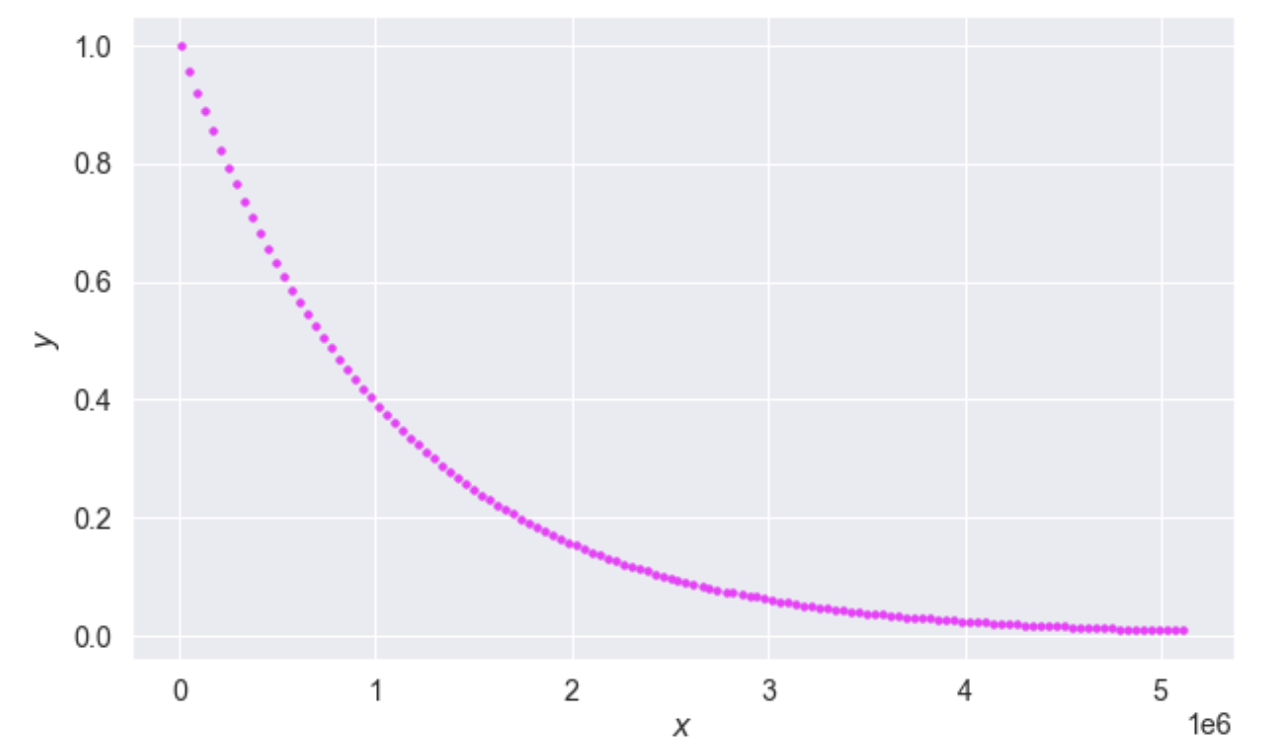
\includegraphics[width=1.0\textwidth]{Рис1}
    \end{figure}


\end{frame}

\begin{frame}
    Для последних 32 точек(четверть) после вычета аппроксимации получаем гистограмму и kde для ошибки

    \begin{figure}[ht]
        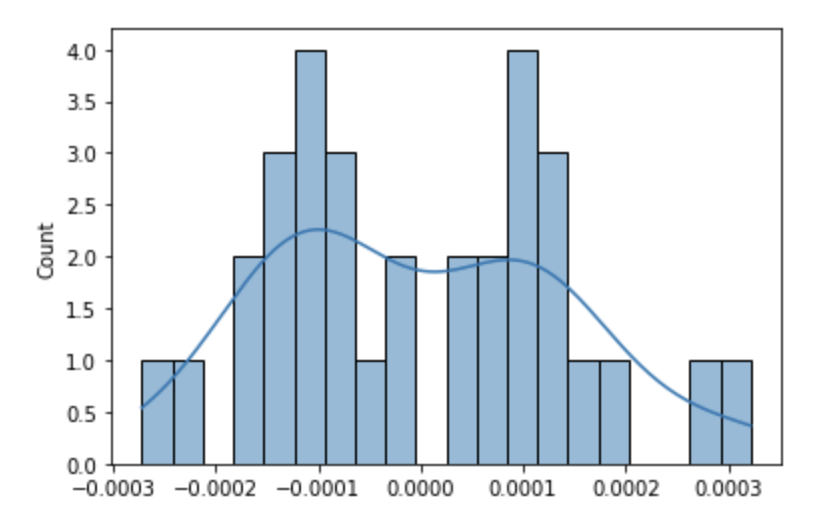
\includegraphics[width=1.0\textwidth]{Гистограмма}
    \end{figure}

\end{frame}


\begin{frame}
    Проверим ошибку на нормальность с помощью критериев Шапиро-Уилка, Жарка-Бера и Лиллиефорса.
    Применим множественную проверку гипотез по методу Холма

    \begin{figure}[ht]
        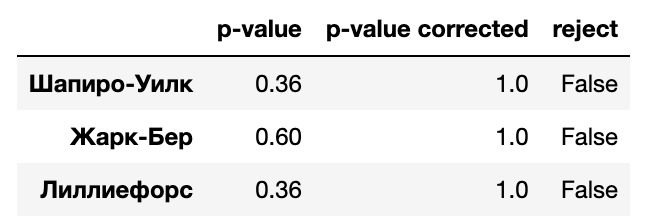
\includegraphics[width=1.0\textwidth]{Таблица1}
    \end{figure}

\end{frame}



\begin{frame}[fragile]
    \textbf{Выводы}

    \begin{itemize}
        \item гипотеза нормальности не отклоняется для всех наборов данных
        \item через ОМП получаем после усреднения на остальных датасетах и проверки нормальности
        параметры ошибки  $Error \sim \mathcal{N}(0, 3.3\cdot 10^{-4})$
        \item для данных с экспоненциальным шагом $Error \sim \mathcal{N}(0, 7.3\cdot 10^{-4})$
        \item синтетические данные будем моделировать с ошибкой $\mathcal{N}(0, 5\cdot 10^{-4})$
    \end{itemize}
\end{frame}

\begin{frame}[fragile]{Параметры экспоненты с наименьшим показателем}
    После логарифмирования $y = \omega \exp(-D x)$ и применения МНК получаем
    $\hat{\ln(y)} = kD + b$, то есть

    \begin{equation}
        \omega = \exp(b), \;\;\; D = -k
    \end{equation}

    Таким образом, в теории можно полностью определить параметры одной из экспонент

    \hspace{1pt}

\end{frame}

    \begin{frame}{Проверка метода}

        Для проверки метода оценки погрешности сгенерировал данные для
        двух экспонент с ошибкой $\mathcal{N}(0, 5\cdot 10^{-4})$

        \hspace{1pt}

        Для первой экспоненты взял $(\omega, D) = (0.1, 1)$, для второй
        параметры пробегали значения

        \begin{itemize}
            \item $\omega \in $ [0.01, 1.0] с шагом 0.01
            \item $D \in $  [1.1, 5.0] с шагом 0.1
        \end{itemize}


        Получил, что в пределах $30\%$ оценка погрешности совпадает с действительным почти для всех точек
        ($< 5$ точек из $\sim 1000$ давали сбой).

        \hspace{1pt}

        Это хороший результат, так как по порядку оценка и погрешность совпадают
    \end{frame}




    \begin{frame}{Доверительная область для двух компонент}

        Критические случаи, когда может быть сложно различить экспоненты:

        \begin{itemize}
            \item близкие показатели экспонент
            \item малая весовая доля одной из экспонент по отношению к другим долям
        \end{itemize}

        Для таких случаев выделим множество параметров для двух экспонент, при котором
        количество экспонент определяется верно. Множество будем строить в координатах
        $\omega_2 / \omega_1$, $D_2/ D_1$


        \hspace{1pt}

        Оценку можно искать либо с помощью метода TRF, либо
        с помощью Dual Annealing + BFGS(две стадии)
        (дал лучшие результаты на сложных случаях для синтетических данных)

    \end{frame}


    \begin{frame}
        За основу возьмём экспоненту с параметрами
        $(0.1, 1)$, будем докидывать к ней экспоненты с параметрами

        \begin{itemize}
            \item $\omega \in $ [0.01, 1.0] с шагом 0.01
            \item $D \in $  [1.1, 2.0] с шагом 0.1
        \end{itemize}

        Качество оценки будем смотреть по метрикам AIC и BIC
        (Akaike Information Criterion и Bayesian Information Criterion)



        \hspace{1pt}

        Будем включать точку в множество, если:
        \begin{itemize}
            \item $\exp(\Delta AIC) > 0.32  \cup  \exp(\Delta BIC > 0.32)$ для 2-ух экспонент
            \item $\exp(\Delta AIC) < 0.32) \cap \exp(\Delta BIC) < 0.32$ для одной и трёх экспонент
        \end{itemize}
    \end{frame}

    \begin{frame}
        \begin{figure}[ht]
            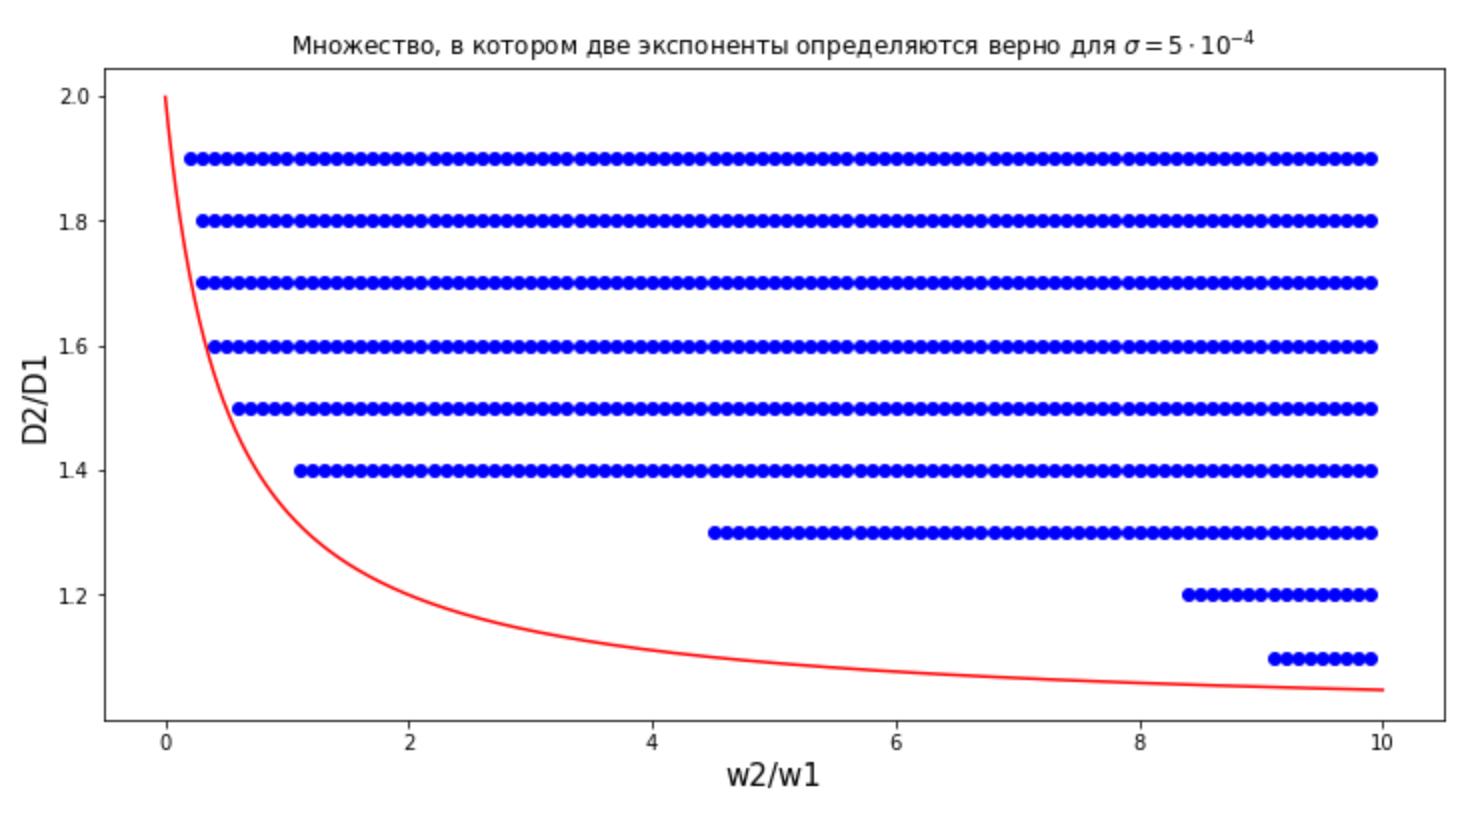
\includegraphics[width=1.0\textwidth]{Множество}
        \end{figure}

        Красная линия на графике задает границу множества
        $G = \{(w_2/w_1, D_2/D_1) : D_2/D_1 > 1 + \frac{0.5}{w_2/w_1 + 0.5} \}$

    \end{frame}

    \begin{frame}
        Пример работы метрики $BIC$ для различного числа экспонент
        \begin{figure}[ht]
            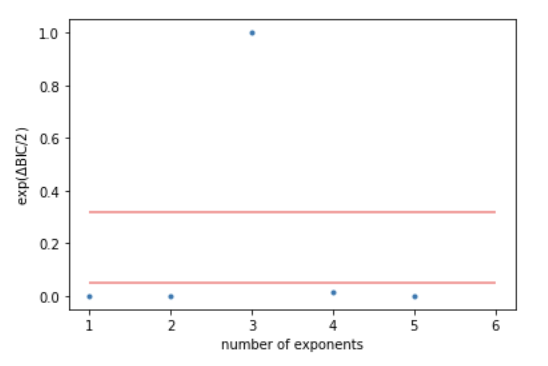
\includegraphics[width=0.8\textwidth]{График2}
        \end{figure}
    \end{frame}


    \begin{frame}{Идея для дальнейшей работы}
        \begin{itemize}

            \item С помощью Монте-Карло моделирования построить
            $2(n-1)$ - мерную область, для которой оценка числа экспонент
            по метрикам AIC и BIC совпадает с их количеством.


            \item Для построения области можно ограничить точки некоторым
            минимальным многоугольником, либо использовать kNN

            \item Если оценка параметров попадает в
            'доверительную область' ,
            считаем, что число компонент определено верно
            \item Квазивеса из библиотеки kmath
            \item Улучшить информационные критерии, ввести объём модели через информацию Фишера

        \end{itemize}

    \end{frame}

\end{document}